\renewcommand*{\arraystretch}{1.1}

\noindent\begin{tabularx}{17cm}{|>{\small \sf}c|X|}
	\hline
	query    & Interactive / complex / 1 \\ \hline
%
	title       & Friends with certain name \\ \hline
%
    pattern     & \hfill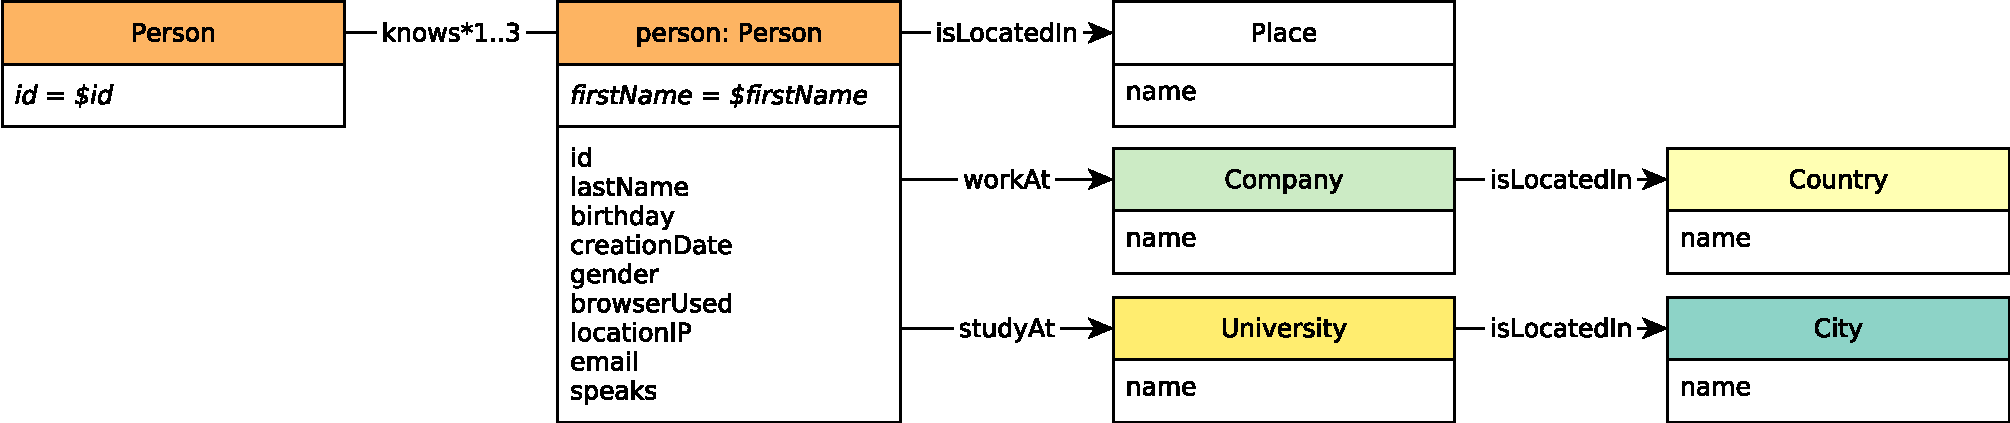
\includegraphics[scale=\patternscale,margin=0cm .2cm]{patterns/interactive-complex-read-01}\hfill\vadjust{} \\ \hline
%
	desc. & Given a start Person, find Persons with a given first name that the
start Person is connected to (excluding start Person) by at most 3 steps
via Knows relationships. Return Persons, including summaries of the
Persons workplaces and places of study.
 \\ \hline
%
	
%
	params.  &
	\vspace{1.1ex}{\begin{tabularx}{14.2cm}{|c|M|m{2cm}|Y|} \hline
	\cellcolor{parameter} \color{white} $\mathsf{1}$ & \varname{Person.id} & \cellcolor{gray!20} \vartype{ID} &  \\ \hline
	\cellcolor{parameter} \color{white} $\mathsf{2}$ & \varname{Person.firstName} & \cellcolor{gray!20} \vartype{String} &  \\ \hline
	\end{tabularx}}\vspace{1.1ex} \\ \hline
%
	
	result      &
	\vspace{1.1ex}{\begin{tabularx}{14.2cm}{|c|M|m{2cm}|c|Y|} \hline
	\cellcolor{result} \color{white} $\mathsf{1}$ & \varname{Person.id} & \cellcolor{gray!20} \vartype{ID} &
	    \texttt{R} &
	     \\ \hline
	\cellcolor{result} \color{white} $\mathsf{2}$ & \varname{Person.lastName} & \cellcolor{gray!20} \vartype{String} &
	    \texttt{R} &
	     \\ \hline
	\cellcolor{result} \color{white} $\mathsf{3}$ & \varname{Person.birthday} & \cellcolor{gray!20} \vartype{Date} &
	    \texttt{R} &
	     \\ \hline
	\cellcolor{result} \color{white} $\mathsf{4}$ & \varname{Person.creationDate} & \cellcolor{gray!20} \vartype{DateTime} &
	    \texttt{R} &
	     \\ \hline
	\cellcolor{result} \color{white} $\mathsf{5}$ & \varname{Person.gender} & \cellcolor{gray!20} \vartype{String} &
	    \texttt{R} &
	     \\ \hline
	\cellcolor{result} \color{white} $\mathsf{6}$ & \varname{Person.browserUsed} & \cellcolor{gray!20} \vartype{String} &
	    \texttt{R} &
	     \\ \hline
	\cellcolor{result} \color{white} $\mathsf{7}$ & \varname{Person.locationIP} & \cellcolor{gray!20} \vartype{String} &
	    \texttt{R} &
	     \\ \hline
	\cellcolor{result} \color{white} $\mathsf{8}$ & \varname{\{Person.email\}} & \cellcolor{gray!20} \vartype{\{String\}} &
	    \texttt{R} &
	     \\ \hline
	\cellcolor{result} \color{white} $\mathsf{9}$ & \varname{\{Person.speaks\}} & \cellcolor{gray!20} \vartype{\{String\}} &
	    \texttt{R} &
	     \\ \hline
	\cellcolor{result} \color{white} $\mathsf{10}$ & \varname{Person-isLocatedIn->Place.name} & \cellcolor{gray!20} \vartype{String} &
	    \texttt{R} &
	     \\ \hline
	\cellcolor{result} \color{white} $\mathsf{11}$ & \varname{\{Person-studyAt->University.name, Person-studyAt->.classYear, Person-studyAt->University-isLocatedIn->City.name\}} & \cellcolor{gray!20} \vartype{\{<String, 32-bit Integer, String>\}} &
	    \texttt{R} &
	     \\ \hline
	\cellcolor{result} \color{white} $\mathsf{12}$ & \varname{\{Person-workAt->Company.name, Person-workAt->.workFrom, Person-workAt->Company-isLocatedIn->Country.name\}} & \cellcolor{gray!20} \vartype{\{<String, 32-bit Integer, String>\}} &
	    \texttt{R} &
	     \\ \hline
	\end{tabularx}}\vspace{1.1ex} \\ \hline
	
%
	sort        &
	\vspace{1.1ex}{\begin{tabular}{|c|l|c|} \hline
	\cellcolor{sort} \color{white} $\mathsf{1}$ & \varname{distanceFromPerson} & \cellcolor{gray!20} $\asc$ \\ \hline
	\cellcolor{sort} \color{white} $\mathsf{2}$ & \varname{Person.lastName} & \cellcolor{gray!20} $\asc$ \\ \hline
	\cellcolor{sort} \color{white} $\mathsf{3}$ & \varname{Person.id} & \cellcolor{gray!20} $\asc$ \\ \hline
	\end{tabular}}\vspace{1.1ex} \\ \hline
	%
	limit       & 20 \\ \hline
	%
	CPs &
	\multicolumn{1}{>{\raggedright}l|}{
	  \chokepoint{1.3}, 
	  \chokepoint{2.1}, 
	  \chokepoint{5.3}
	  } \\ \hline
	%
    relevance &
      \small This query is a representative of a simple navigational query. It looks for paths of length one, two or three through
the knows relation, starting from a given Person and ending at a Person with a given name. It is interesting for several
aspects. First, it requires for a complex aggregation, that is, returning the concatenation of universities, companies,
languages and email information of the person. Second, it tests the ability of the optimizer to move the evaluation of
sub-queries functionally dependant on the Person, after the evaluation of the top-k. Finally, performance is
highly sensitive to properly estimating the cardinalities in each transitive path, and paying attention not to explode
already visited Persons.
 \\ \hline%
\end{tabularx}
\vspace{2ex}